\section{数据特征与公共物理模型}
\subsection{数据来源与统一口径}
节点、货箱、运输机、中继机和通信参数分别由五份工作簿提供，地形由30米DEM描述\cite{Data2026}。表\ref{tab:inputs}给出参与建模的对象规模。逐箱货箱清单作为分配的最小粒度，需求汇总表用于交叉核对；不能同时把两张表中的需求累加。
\begin{table}[htbp]\centering
\caption{标准场景的数据与资源构成}\label{tab:inputs}
\begin{tabularx}{\linewidth}{lYl}\toprule
对象 & 计算用途 & 规模\\\midrule
调度节点 & 航段、投送与网关定位 & 1个中心、15个服务区\\
逐箱需求 & 不可拆分配送与逐箱时限 & 80箱、53条汇总记录\\
运输无人机 & 机型选择与实体调度 & A/B/C共8架\\
运输电池 & 同型共享与充电周转 & A/B/C共14组\\
中继设备 & 空中接入与网关回传 & 2架、6组能源组件\\
DEM & 最高地形与视线遮挡 & $1309\times1486$像元\\
\bottomrule\end{tabularx}\end{table}

节点与需求空间关系见图\ref{fig:service-map}。点位决定飞行距离，点面积反映需求质量；二者共同影响组批，但尚不能据此判断某节点需要多少架次，因为安全载荷还受爬升和返航余量约束。
\begin{figure}[htbp]\centering
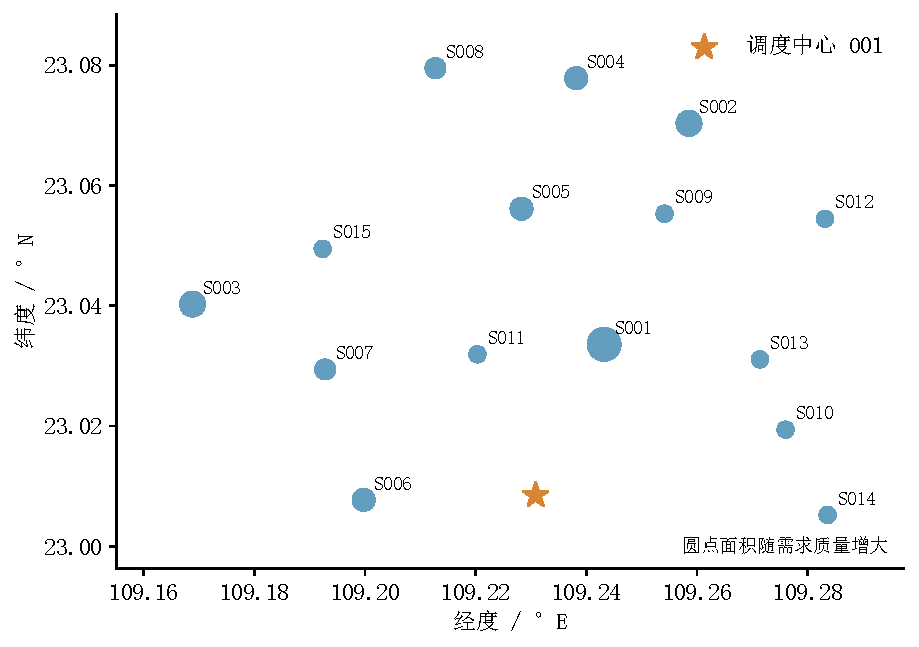
\includegraphics[width=.86\linewidth]{figures/data/raw_service_map.pdf}
\caption{调度中心与服务区分布：依据附件节点坐标与逐区需求绘制}
\label{fig:service-map}\end{figure}

\subsection{需求结构与时限分类}
逐箱统计得到总质量758 kg、总体积2.011 m$^3$。其中医疗箱16箱，首批保障箱30箱，二者交集15箱，故具有至少一种硬时限要求的货箱数为
\begin{equation}N_{hard}=16+30-15=31.\label{eq:hard-count}\end{equation}
余下49箱使用期望送达时间计算软迟到。交集不能重复计数：同一货箱既为医疗物资又为首批保障时，应取两个适用截止时刻的较小值，而不是将其视为两项配送任务。

图\ref{fig:demand}同时展示需求质量和硬软时限构成。这一组合图把载荷规模与时间紧迫程度并列，便于识别“质量较大”与“必须尽早送达”并非同一概念。图\ref{fig:deadlines}进一步区分仅医疗、仅首批、两者兼有和一般物资；相同坐标的样本合并表示，避免重叠掩盖数量。

从逐区统计可见，S001拥有15箱、154 kg需求，约占总质量的20.3\%；S009至S015各有3箱、25 kg需求。S001的硬时限箱为3箱，其余服务区均为2箱，说明需求质量的差异明显大于硬时限箱数量的差异。调度时需要既给各区配置早期保障，又为大需求节点安排后续运力，不能仅按总质量大小排序服务。
\begin{figure}[htbp]\centering
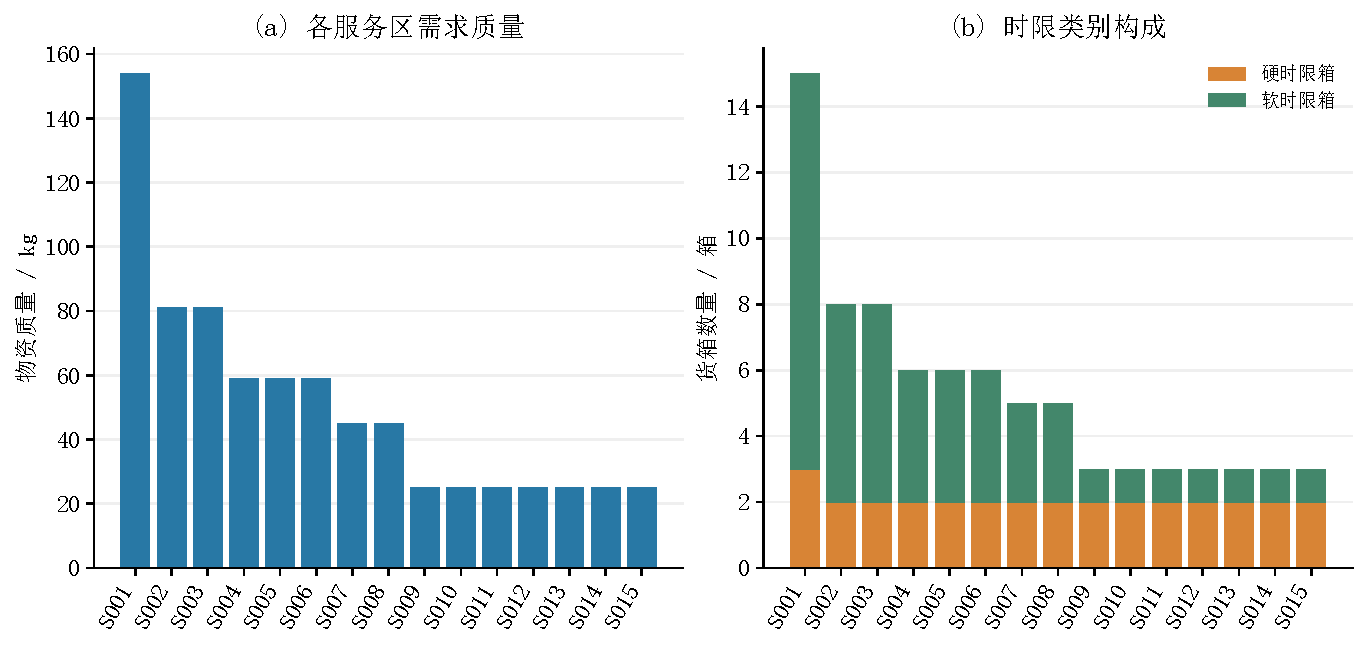
\includegraphics[width=\linewidth]{figures/data/raw_demand_composition.pdf}
\caption{各服务区的需求质量及硬软时限货箱构成}\label{fig:demand}\end{figure}
\begin{figure}[htbp]\centering
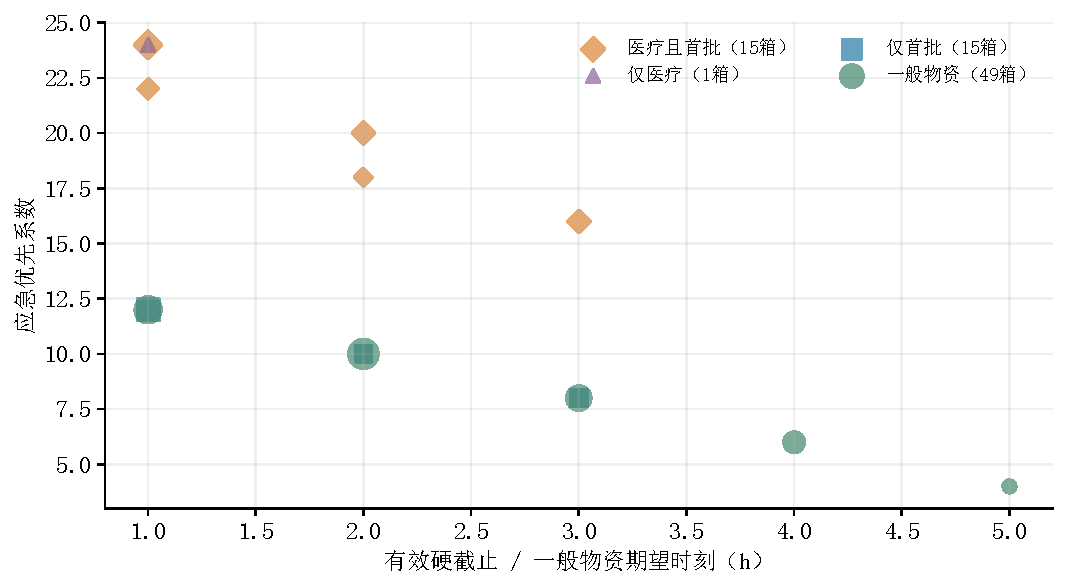
\includegraphics[width=.9\linewidth]{figures/data/raw_deadline_classes.pdf}
\caption{时限与优先系数：硬时限箱采用有效截止，一般物资采用期望时刻；点面积随同坐标箱数增大}\label{fig:deadlines}\end{figure}

\subsection{异构机型与能源库存}
三类机型的容量和库存见表\ref{tab:types}。C型具有较大的额定载质量和体积，但不能仅凭容量判定其在所有节点最优：不同载荷下的等效航程、爬升质量和实体数量均会影响调度。共享电池总数包含初始装机与备用电池，不能再额外加上实体机数量。
\begin{table}[htbp]\centering
\caption{运输机型容量与同型资源库存}\label{tab:types}
\begin{tabular}{lrrrrr}\toprule
机型 & 载质量/kg & 体积/m$^3$ & 能量/kWh & 实体机/架 & 电池/组\\\midrule
A & 25 & 0.060 & 4.5 & 4 & 6\\
B & 30 & 0.073 & 4.0 & 2 & 4\\
C & 80 & 0.250 & 8.0 & 2 & 4\\\bottomrule
\end{tabular}\end{table}

\subsection{航段、地形净空与飞行时间}
设节点经纬度为$(\lambda_i,\varphi_i)$，采用局部米制近似计算节点对距离：
\begin{equation}
d_{ij}=R\sqrt{\cos^2\!\left(\frac{\varphi_i+\varphi_j}{2}\right)(\lambda_j-\lambda_i)^2+(\varphi_j-\varphi_i)^2},
\end{equation}
其中角度以弧度计，$R=6371008.8$ m。该距离只对应水平巡航段；垂直运动在飞行时间中分别计算。

令$\mathcal C_{ij}$为航段水平直线实际经过的DEM像元集合，$H_c$为像元地面高程。题设要求的巡航海拔为
\begin{equation}
H_{ij}^{c}=\max_{c\in\mathcal C_{ij}}H_c+50.\label{eq:terrain}
\end{equation}
计算时应按地理配准及像元边界确定$\mathcal C_{ij}$，覆盖短距离穿越的像元；固定步长采样点的最大值并不天然等于经过像元的最大值。此处给出模型定义，具体像元遍历和边界处理仍需按该定义复验。

调度中心作业海拔为给定地面海拔，服务区作业海拔为地面海拔加30 m。由此定义
\begin{equation}
h_{ij}^{+}=\max(0,H_{ij}^{c}-H_i^{op}),\qquad
h_{ij}^{-}=\max(0,H_{ij}^{c}-H_j^{op}).
\end{equation}
每一航段的时间均为爬升、水平巡航和下降时间之和：
\begin{equation}
t_{gij}=\frac{h_{ij}^{+}}{v_g^{up}}+\frac{d_{ij}}{v_g^{cr}}+\frac{h_{ij}^{-}}{v_g^{down}}.\label{eq:leg-time}
\end{equation}
多点任务在每次交付后从服务区作业高度重新爬升，不能将多个访问点之间的飞行简化为一次长距离等高巡航。

\subsection{载荷相关能耗与返航约束}
附件的等效航程随当前载荷变化：
\begin{equation}
L_g(q)=L_g^0-(L_g^0-L_g^F)\left(\frac{q}{Q_g}\right)^{3/2},\quad 0\le q\le Q_g.
\label{eq:range}
\end{equation}
按前述能耗解释，水平航段能耗和爬升附加能耗分别为
\begin{equation}
E_{gij}^{hor}(q)=E_g^{use}\frac{d_{ij}}{L_g(q)},\qquad
E_{gij}^{up}(q)=\frac{(m_g^0+q)g_0h_{ij}^{+}}{3.6\times10^6\eta_g^{up}}.
\label{eq:energy}
\end{equation}
式中$g_0=9.80665$ m/s$^2$，分母$3.6\times10^6$把焦耳换算为kWh。下降效率取0时，不另计下降附加能耗，也不作能量回收。货箱交付后，从剩余载荷中扣除其质量；返航通常为空载，不能把起飞载荷代入整个架次。

架次$r$的总能耗和返航荷电状态满足
\begin{equation}
E_r=\sum_{(i,j)\in r}\bigl(E_{gij}^{hor}(q_{ij})+E_{gij}^{up}(q_{ij})\bigr),
\quad SOC_r^{end}=1-\frac{E_r}{E_g^{use}}\ge\rho_g.
\label{eq:soc}
\end{equation}

\subsection{两阶段充电与资源再次可用}
令返航SOC为$s$，从$s$充至满电所需时间按题面规则计算：
\begin{equation}
T^{chg}(s)=T^{full}\begin{cases}
0.65(0.9-s)/0.9+0.35,&0\le s<0.9,\\
0.35(1-s)/0.1,&0.9\le s\le1.
\end{cases}\label{eq:charge}
\end{equation}
该式在$s=0.9$处连续，在$s=1$时为0。每组电池返航后单独记录SOC和充电结束时刻，同型电池可在不同实体机之间调配，异型电池不得混用。不同能源资源可以并行充电，因此在未给出充电工位限制的条件下，不额外引入单工位排队。
